\chapter{Introduction}
\label{cha:chapter_1}

This chapter introduces the research context by highlighting the significance of \ac{dpp} systems and their critical role within the \ac{ce} (\Cref{sec:motivation}). It further identifies and discusses the primary challenges and research gaps currently hindering the widespread adoption of \ac{dpp} systems (\Cref{sec:problem_statement}). Subsequently, the objectives of this thesis are clearly articulated (\Cref{sec:objectives}), followed by an overview of the thesis structure (\Cref{sec:thesis_structure}).


\section{Motivation}
\label{sec:motivation}

The escalating consumption of raw materials and the increasing challenges associated with waste management have necessitated a shift from a Linear Economy to a \acrlong{ce}. The \acrlong{ce} aims to minimize resource usage and waste generation by closing material loops and prolonging product lifecycles \autocite{EllenMacArthurFoundation.2015}. A fundamental enabler of this transition is the \acrlong{dpp}, which facilitates the traceability, transparency, and sustainable lifecycle management of products. The \acrlong{eu}'s (\acrshort{eu}'s) \ac{espr} has introduced \ac{dpp}s as a policy tool to standardize product information, especially sustainability-related information, and promote environmentally responsible product design \autocite{Garcia.2024}. By embedding essential product information such as material composition, carbon footprint, and end-of-life treatment, \ac{dpp}s enable informed decision-making across value chains \autocite{Psarommatis.2024}.

A \ac{dpp} is defined as a structured digital dataset accompanying a product throughout its lifecycle, containing essential data on sustainability, repairability, recyclability, and compliance with environmental standards . The importance of such digital passports arises from both regulatory pressures, such as the \ac{espr}, and increasing market demands for transparency in sustainability practices. \autocite{EuropeanParliamentandCouncil.2024}

Despite the regulatory push and conceptual advancements, practical implementation of \ac{dpp} systems remains complex. Industries are faced with challenges in standardization, interoperability, data security, and integration with existing digital infrastructures \autocite{Ducuing.2023}. Currently, there is a surge of ongoing research and multiple initiatives aiming to implement \ac{dpp} solutions, but no widely accepted technological approach has surfaced so far. Various industry-wide initiatives, such as CIRPASS and Catena-X, aim to address these challenges, but a unified and scalable framework is still lacking. The heterogeneity of data governance models and the absence of universally accepted protocols create fragmentation, further hindering industry-wide adoption. Many existing approaches remain isolated or sector-specific, with varying degrees of integration capability, data quality, and regulatory alignment \autocite{Jansen.2023,Jousse.2024}.


\section{Problem Statement}
\label{sec:problem_statement}

Although the concept of \acrlong{dpp}s has gained significant traction, its practical realization remains ambiguous. The current landscape is characterized by divergent technological approaches, lack of interoperability, and regulatory uncertainties in the face of evolving \ac{eu} regulations \autocite{Adisorn.2021}. Several critical problems stand out as main obstacles for the widespread adoption of \ac{dpp} systems:

\begin{itemize}
    \item \textbf{Lack of a Unified Technology Framework:} Existing \ac{dpp} implementations are often sector-specific and do not follow a common reference architecture \autocite{Jansen.2023}. This fragmentation prevents seamless data exchange across supply chains.
    \item \textbf{Regulatory Compliance Uncertainty:} While \ac{espr} outlines mandatory data requirements, there are still many open questions, missing standards and continuously evolving regulations. \autocite{Garcia.2024}
    \item \textbf{Technology Selection Challenges:} The absence of a systematic evaluation framework makes it difficult to determine which foundational technologies (Blockchain, Cloud, Digital Twins, etc.) are most suitable for different \ac{dpp} use cases. \autocite{Nowacki.2023}
    \item \textbf{Scalability and Industry Adoption Barriers:} \ac{sme} and industries with complex global supply chains struggle with the costs and technical overhead associated with \ac{dpp} implementation. \autocite{Psarommatis.2024}
\end{itemize}

Furthermore, digitalization disparities across industries pose challenges for broad adoption, as companies vary significantly in their ability to implement data-driven solutions. Beyond selecting core technologies, \ac{dpp} implementation requires designing comprehensive system architectures. The interplay between consumer-facing transparency and internal supply chain management further complicates system design. The lack of standardized data governance models magnifies these challenges and complicates interoperability between different stakeholders, while sector-specific solutions continue to create fragmentation. 


\section{Objectives}
\label{sec:objectives}

Given the identified challenges and the upcoming regulatory mandates for \ac{dpp}s under the \ac{espr} (\ac{eu} Regulation 2024/1781), it is paramount to establish a structured methodology for \ac{dpp} system design. Most importantly, the regulation confirms that \ac{dpp}s will progressively extend beyond initially targeted sectors to encompass all regulated product categories, effectively impacting all manufacturers subject to \ac{eu} product regulations \autocite{EuropeanParliamentandCouncil.2024}. This broad scope reinforces the necessity of a structured, scalable approach capable of accommodating cross-sectoral adoption and full economy-wide integration across diverse manufacturing domains.

Taking into account the complexity of \ac{dpp} systems, which span regulatory, technical, and sector-specific challenges, this research aims to bridge the gap between conceptual frameworks and practical, scalable implementations.

To achieve this, the thesis is structured into the following specific objectives, each sequentially building upon the insights derived from the previous stages:

\begin{enumerate}[label=\textbf{O\arabic*}, itemsep=\baselineskip]
    \item \textbf{Analysis of the State of the Art in \acrlong{dpp} Systems}
    \begin{itemize}
        \item Conduct a systematic review of the literature on \acrlong{dpp}s, analyzing their conceptual foundations, current definitions, and essential components.
        \item Critically examine existing regulatory frameworks (particularly \ac{espr} and related \ac{eu} policies) and their implications for \ac{dpp} system requirements.
        \item Identify and categorize key enabling technologies.
        \item Identify the current challenges and research gaps.
    \end{itemize}

    \item \textbf{Empirical Analysis of Industry Initiatives and Technological Trends}
    \begin{itemize}
        \item Conduct a quantitative data analysis of industry initiatives, analyzing the adoption trends and technological choices of real-world implementations.
        \item Identify industry patterns in technology selection, capturing sector-specific preferences, common technological approaches, and deviations across sectors.
    \end{itemize}

    \item \textbf{Expert Interviews and Derivation of of a Structured Evaluation Framework}
    \begin{itemize}
        \item Conduct semi-structured expert interviews to gain first-hand qualitative insights into practical industry challenges, priorities, and real-world constraints faced by stakeholders the ecosystem.
        \item Derive comprehensive functional and technological requirements and limitations directly from insights provided by experts, enhancing and building upon findings from previous literature and empirical analysis.
        \item Define and validate a set of \ac{kpi}s with industry experts, forming a robust basis for conducting \ac{uva} evaluations.
    \end{itemize}

    \item \textbf{Development of a Generic \ac{dpp} System Design Model}
    \begin{itemize}
        \item Conduct a morphological analysis integrating the state-of-the-art research, empirical insights, and expert input to construct a morphological box of \ac{dpp} system architecture.
        \item Utilize the morphological box to develop a generic model for systematically deriving technological architectures for \ac{dpp} solutions.
    \end{itemize}

    \item \textbf{Design and Implementation of a \ac{dpp} Prototype}
    \begin{itemize}
        \item Demonstrate practical feasibility by selecting and implementing a suitable technological architecture derived from the generic \ac{dpp} model.
        \item Develop a modular prototype adhering to the selected architectural pathway, clearly reflecting insights from industry practices, expert evaluations, and regulatory compliance requirements.
        \item Ensure prototype flexibility, scalability, and practical relevance by implementing back-end functionalities and front-end interfaces aligned explicitly with the previously established evaluation criteria.
    \end{itemize}

    \item \textbf{Critical Evaluation and Validation of the Developed Solution}
    \begin{itemize}
        \item Validate and critically evaluate the prototype implementation against the developed evaluation framework, specifically applying the \ac{uva} to measure and illustrate the practical effectiveness of the implemented solution.
        \item Synthesize key findings, providing recommendations for future research and practical industry applications.
    \end{itemize}
\end{enumerate}

\begin{figure}[htbp]
  \centering
  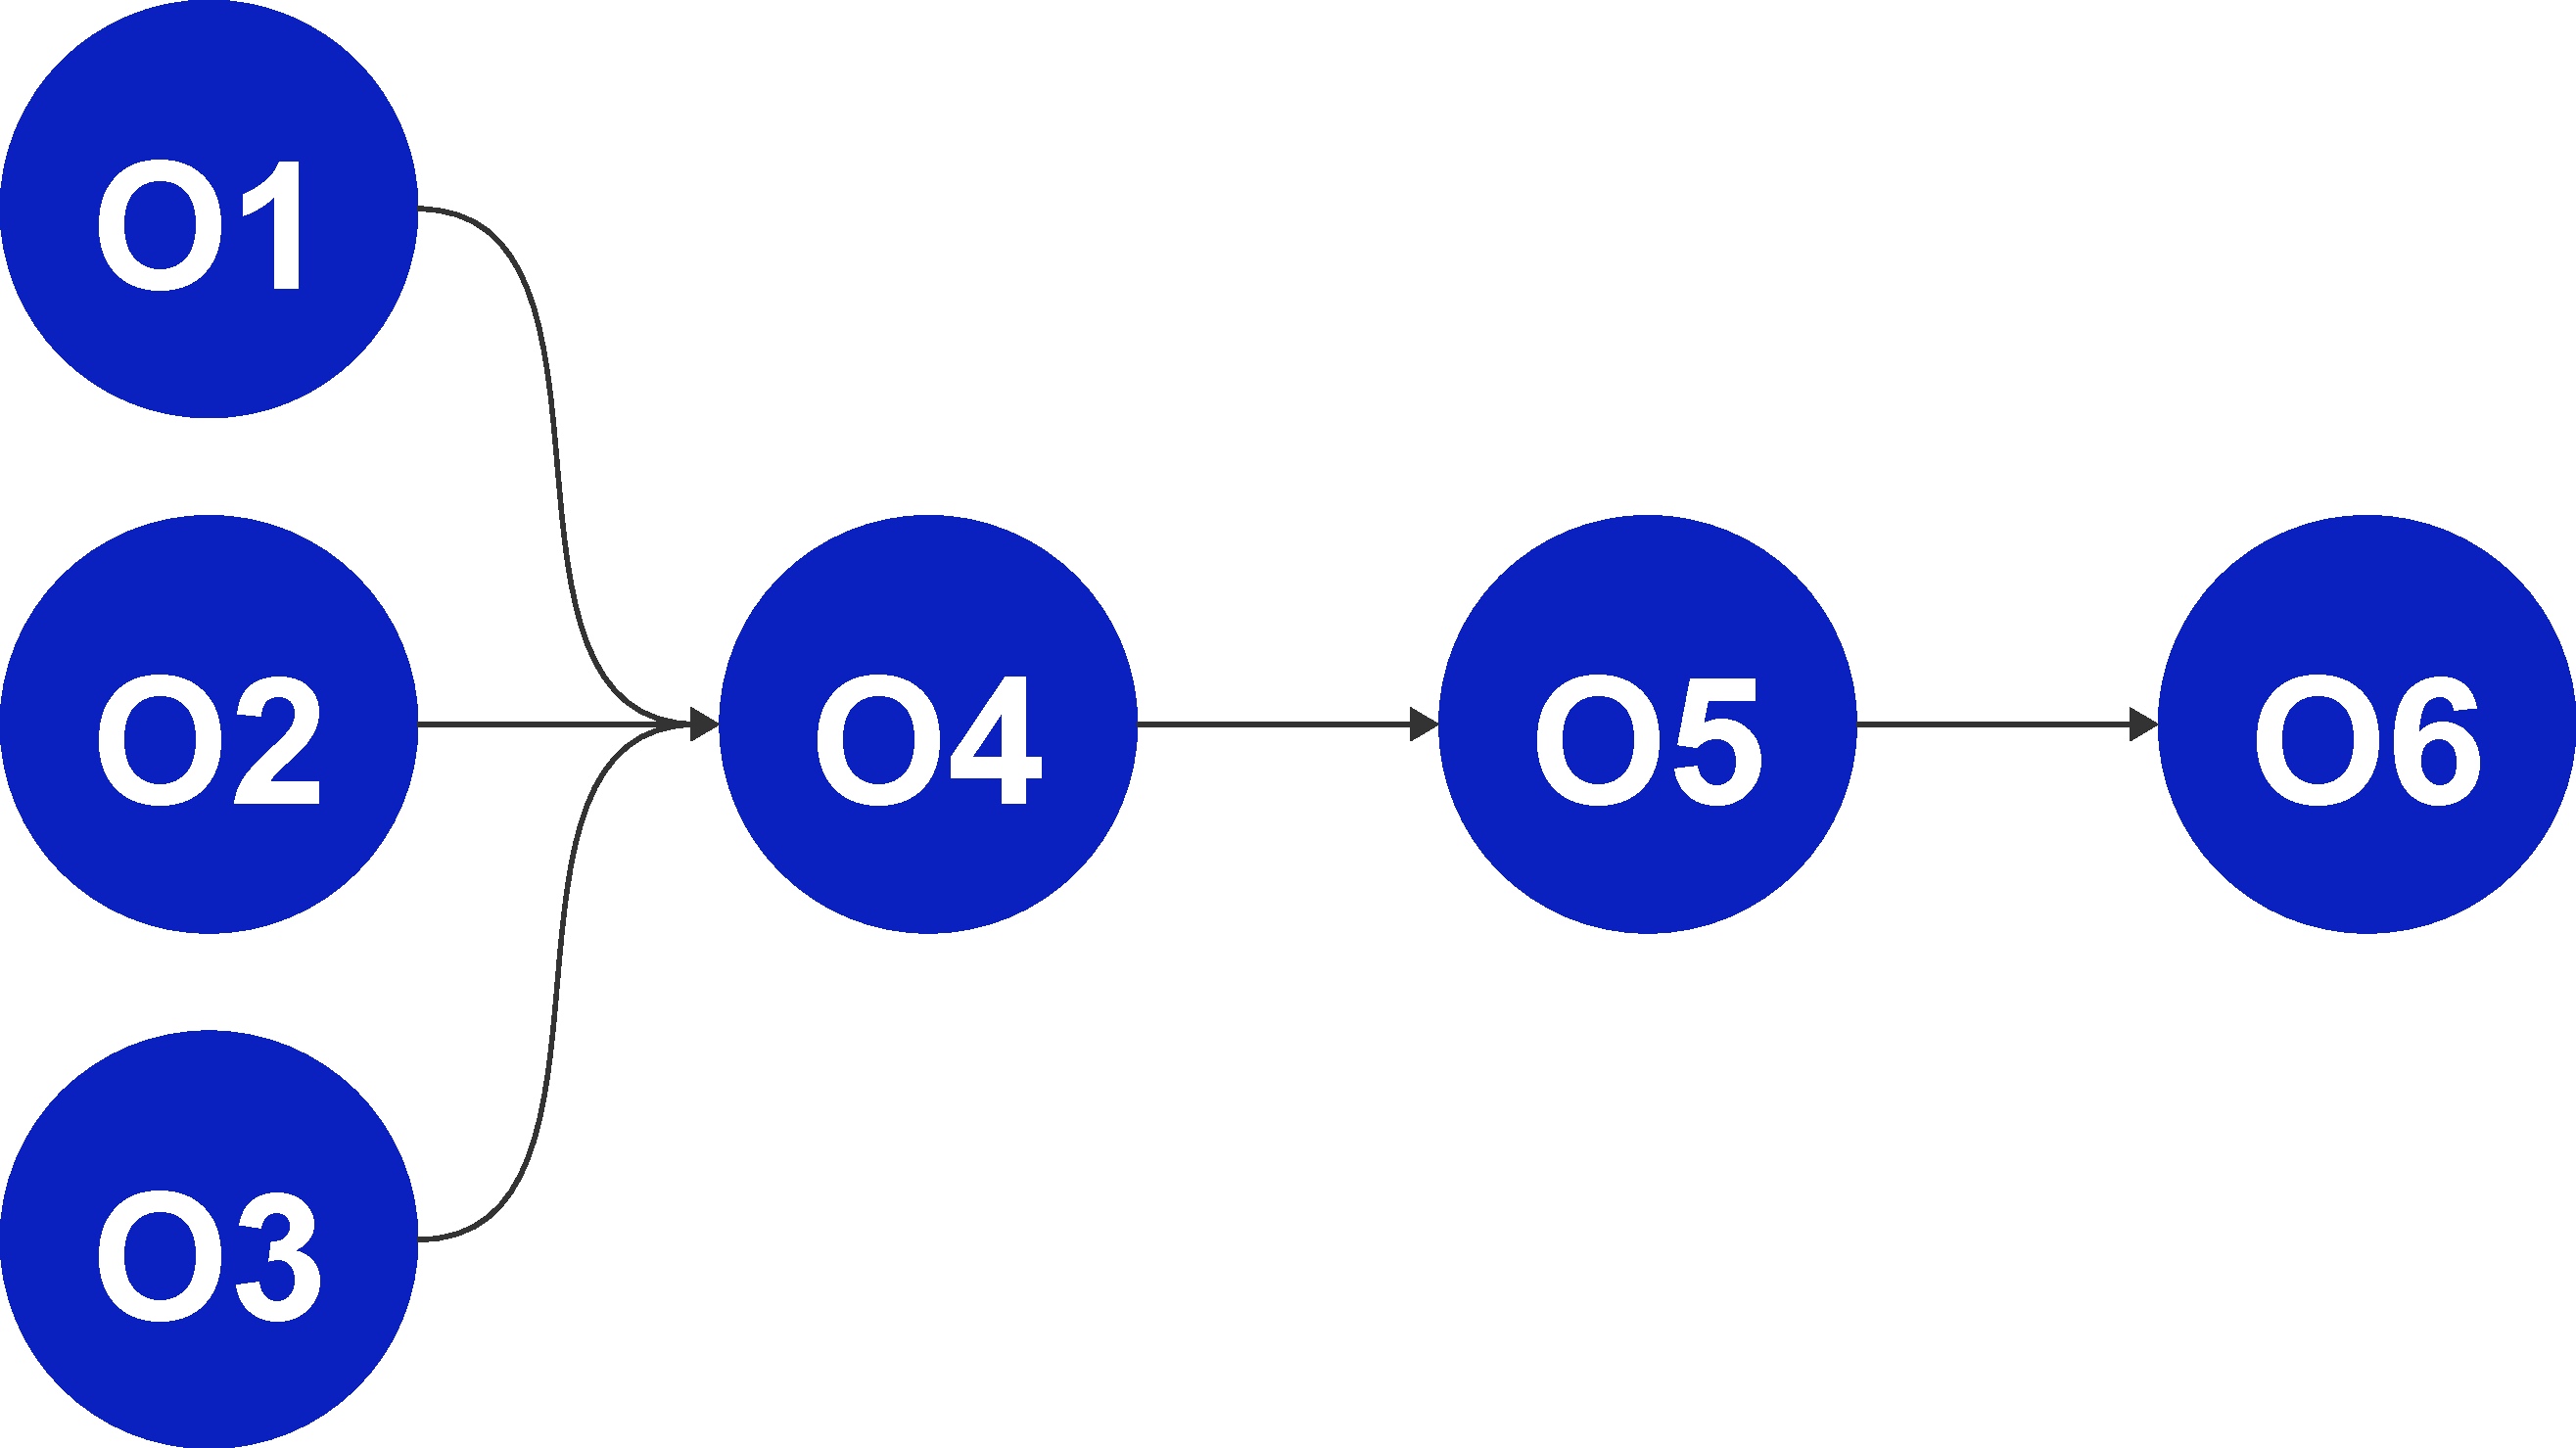
\includegraphics[width=0.8\textwidth]{figures/objectives_diagram.pdf}
  \caption{%
    \textit{Schematic representation of the logical flow of objectives} 
  }
  \label{fig:objectives_flow}
\end{figure}

\section{Thesis Structure}
\label{sec:thesis_structure}

The structure of this thesis, comprising six chapters along with their corresponding objectives, is illustrated in \cref{fig:thesis_structure}. Each chapter systematically contributes to the development of a structured evaluation framework for \acrlong{dpp} technological solutions, a formulation of a a generic model for deriving \ac{dpp} architectures and the implementation of a \acrlong{poc} prototype.

\Cref{cha:chapter_1} introduces the research context, problem statement, objectives, and thesis structure. \Cref{cha:chapter_2} provides the literature review, touching upon conceptual foundations, regulatory frameworks, and enabling technologies. This chapter establishes the theoretical background, presents a theoretical analysis of the state of the art in \ac{dpp} systems and identifies critical research gaps. \Cref{cha:chapter_3}  presents an empirical data analysis of industry initiatives and technological trends based on data from the CIRPASS "DPP-related Initiatives Dataset". \Cref{cha:chapter_4} builds upon previous findings by developing a structured evaluation framework for assessing \ac{dpp} technological architectures. It begins with the design and execution of expert interviews, detailing the interview guide setup, methodology, and key insights gathered from the experts. The interview findings inform a \acrlong{uva}, where the expert-provided scores are used to derive importance weights for predefined \ac{kpi}s. The chapter culminates in the development of a generic model for deriving \ac{dpp} technological architectures, integrating regulatory constraints, industry insights, and evaluation criteria to guide scalable and flexible \ac{dpp} system design. \Cref{cha:chapter_5} applies the generic model to derive a system design pathway and proceed with the implementation of a robust pilot system. Conclusively, \Cref{cha:chapter_6} critically discusses the research outcomes and evaluates the pilot project by validating it against the structured evaluation framework developed in \Cref{cha:chapter_4}. The chapter further discusses key limitations and gives directions for future research.

\begin{figure}[htbp]
  \centering
  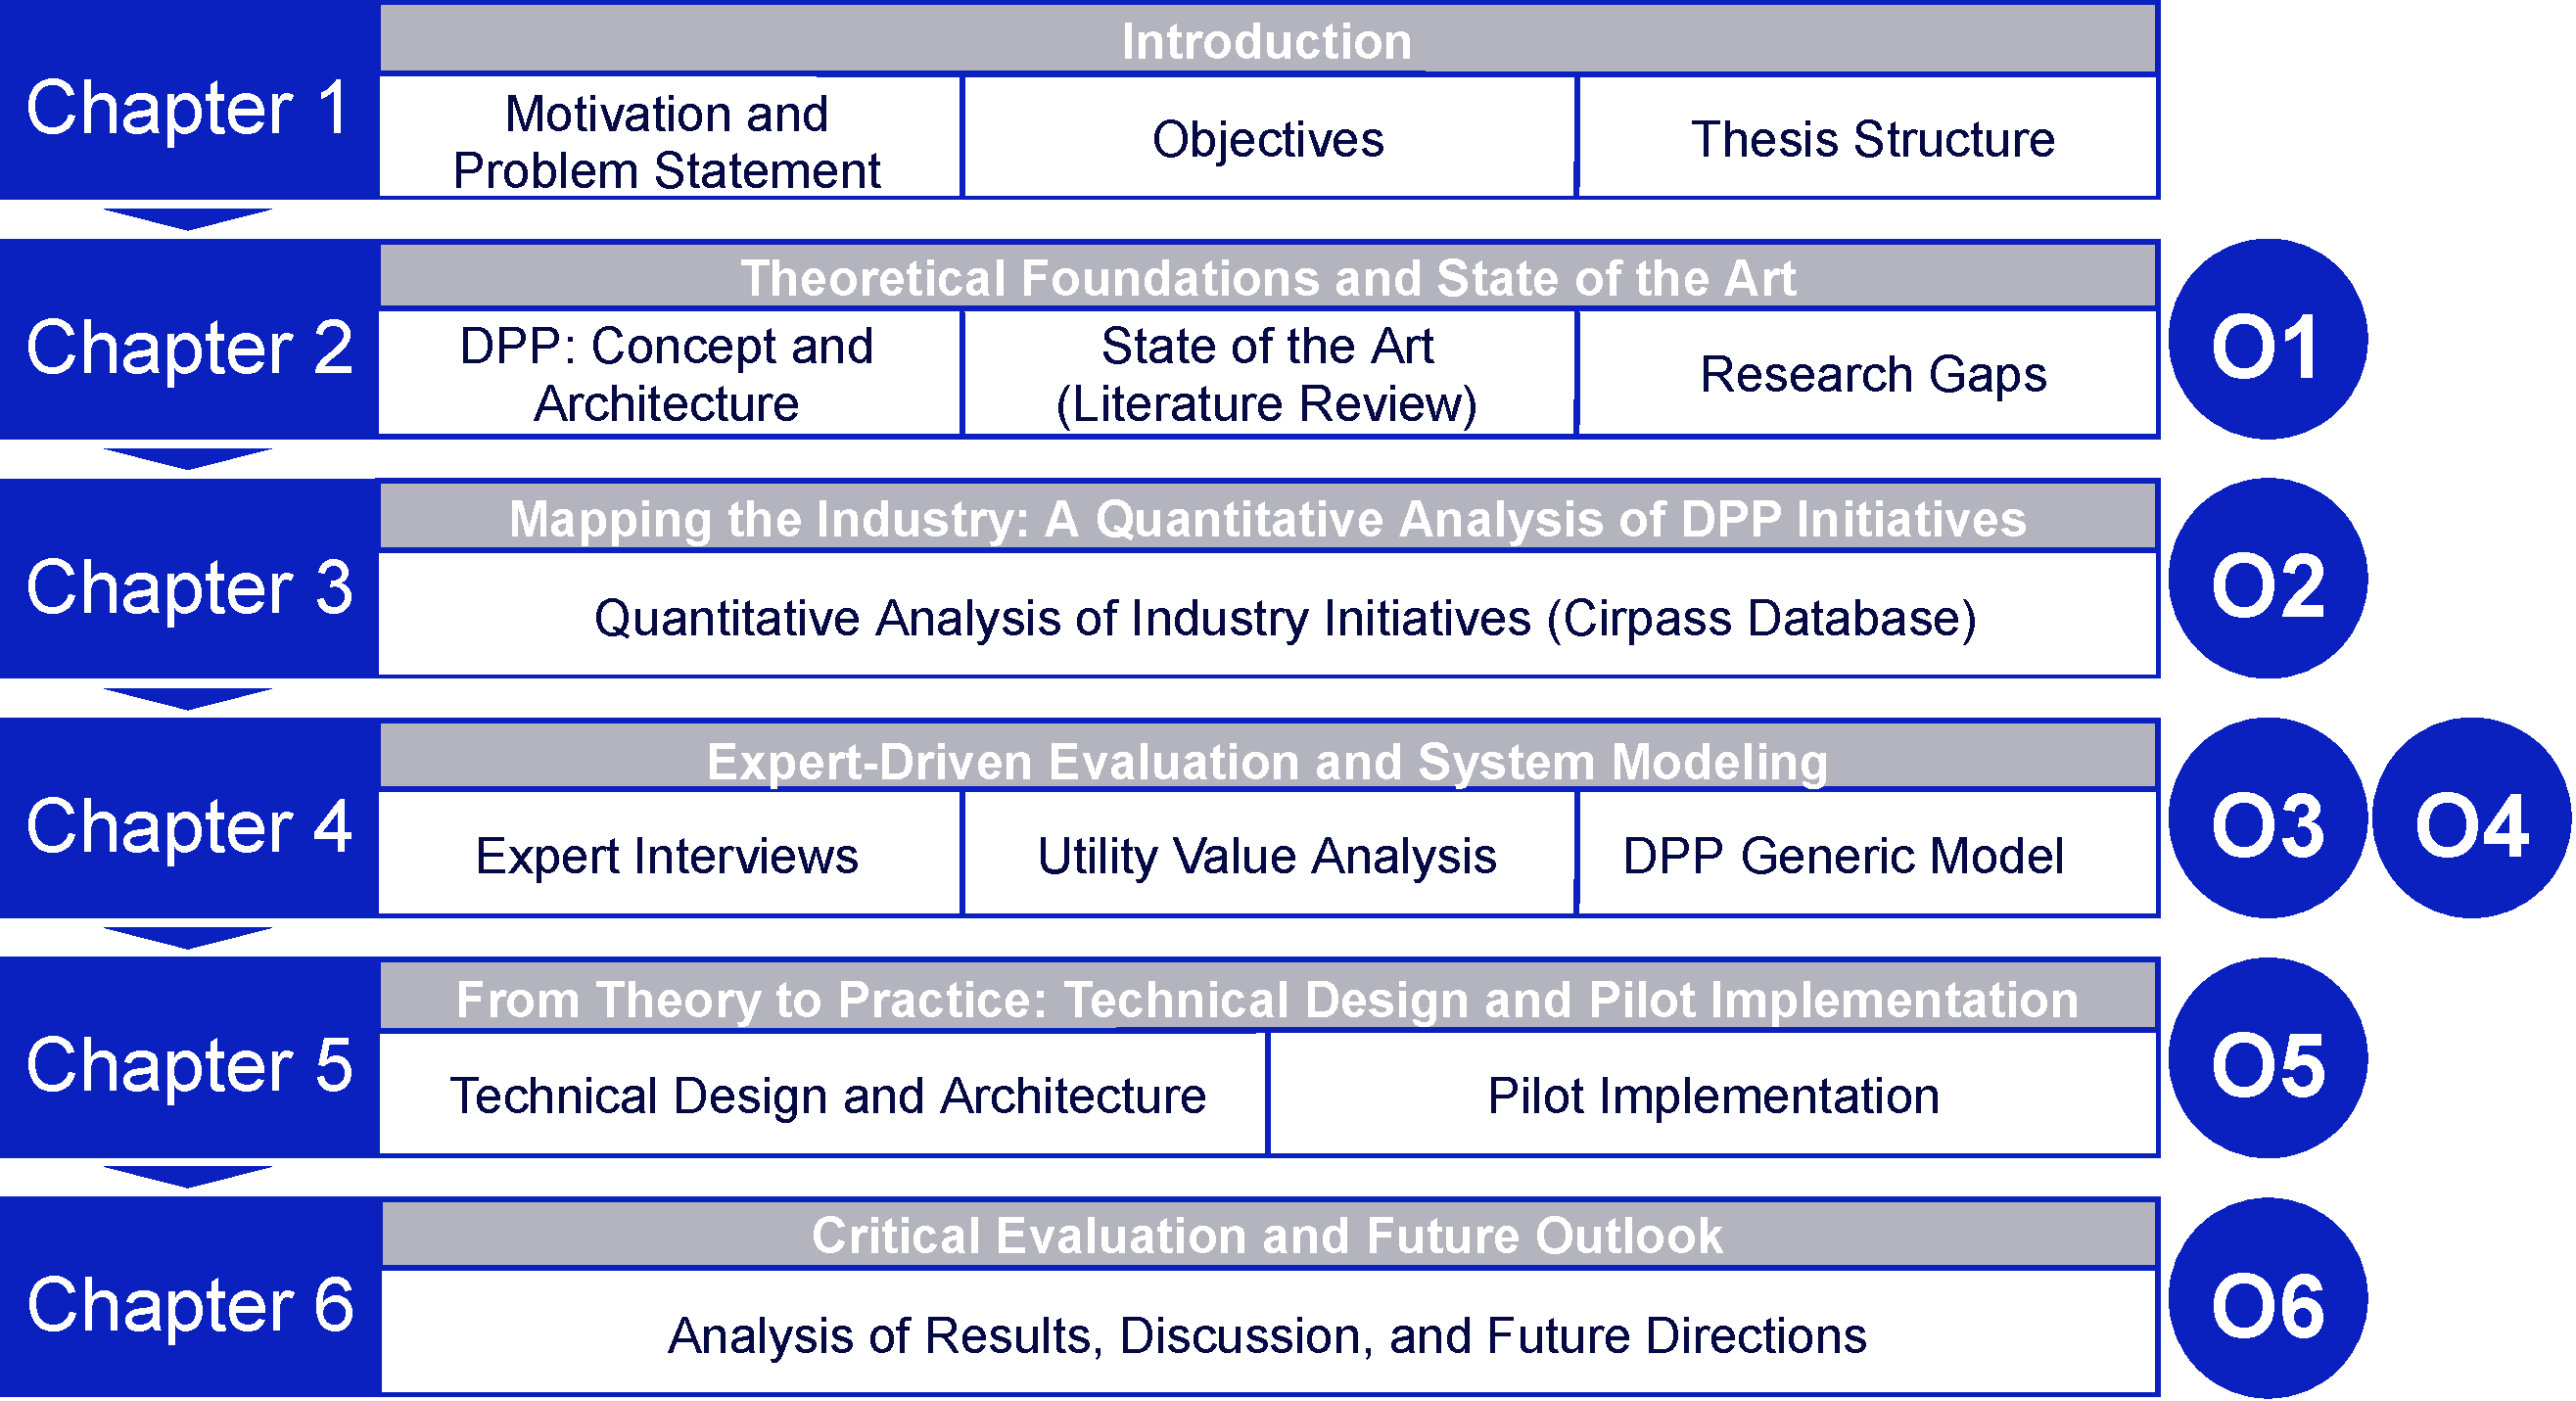
\includegraphics[width=\textwidth]{figures/thesis_structure.pdf}
  \caption{%
    \textit{Structure of the Thesis} 
  }
  \label{fig:thesis_structure}
\end{figure}